\documentclass{beamer}
%\usetheme{Frankfurt}
%\usecolortheme{dove}
\usetheme[faculty=we]{UniversiteitGent}
\useinnertheme{circles}
\setbeamertemplate{navigation symbols}{}

\usepackage{media9}
\usepackage{graphicx}
\usepackage[T1]{fontenc}
\usepackage[utf8]{inputenc}
%\usepackage{cmbright}
\usepackage{lmodern}
\usepackage[outputdir=.texpadtmp]{minted}
\usepackage{siunitx}

\usepackage{silence}
\WarningFilter{latexfont}{Font shape}
\WarningFilter{latexfont}{Some font}

\usepackage{remreset}% tiny package containing just the \@removefromreset command
\makeatletter
\@removefromreset{subsection}{section}
\makeatother
\setcounter{subsection}{1}

\DeclareRobustCommand{\cpluspluslogo}{\hbox{C\hspace{-0.15ex}\protect\raisebox{0.5ex}{\protect\scalebox{0.67}{++}}}}

\title{\LARGE\textbf{N-body simulations}}
\author{\texorpdfstring{Kevin Canters, Kwinten De Backer,\\ Tamas Gommers en Johannes Weytjens}{Kevin Canters, Kwinten De Backer, Tamas Gommers en Johannes Weytjens}}
\date{15 december, 2015}
\begin{document}

\begin{frame}
\maketitle
\end{frame}

\section{\texorpdfstring{\cpluspluslogo}{C++} code}
\begin{frame}
\frametitle{\thesection. \insertsection}
\framesubtitle{General principles}
\begin{itemize}[<+->]
	\item Maximize readability by hiding \texttt{for} loops
	\item Optimize for speed keeping the first rule in mind
	\item Gragg-Bulirsch-Stür should adjust timestep if necessary
	\item Provide a nice user interface
\end{itemize}
\end{frame}

\begin{frame}
\frametitle{\thesection. \insertsection}
\framesubtitle{Optimalizations}
\begin{itemize}
	\item<1-> Pass classes by reference if it doesn't obstruct readability
	\item<1-> \texttt{valarray} and \texttt{array} instead of \texttt{vector}
	\begin{itemize}
		\item<2-> speed record: Burrau problem with RK in \alert{\SI{0.2}{\second}}
	\end{itemize}
	\item<3-> \texttt{[]} operator instead of \texttt{.at()}
	\item<3-> \texttt{size\textunderscore t valarray.size()}
	\item<3-> Loops over all possible pairs are symmetric 
\end{itemize}

	
\end{frame}

%\begin{frame}[fragile]
%\begin{minted}{cpp}
%valarray<Vec> getPositions(const valarray<Star>& stars)
%{
%    size_t size = stars.size();
%    valarray<Vec> positions(size);
%
%    for(size_t i = 0; i < size; ++i)
%    {
%        positions[i] = stars[i].position();
%    }
%    return positions;
%}	
%\end{minted}
%\end{frame}
%
%\begin{frame}[fragile]
%\begin{minted}{cpp}
%valarray<Star> modifiedMidpoint(valarray<Star> stars, ...)
%{
%    valarray<Vec> xi, xi_min, xi_plus;
%    valarray<Vec> vi, vi_min, vi_plus;
%    valarray<double> masses = getMasses(stars);
%    
%    for(size_t i = 0; i < n - 1; ++i) 
%    {
%        xi_plus = xi_min + 2 * h * vi; 
%        vi_plus = vi_min + 2 * h * driver(xi, masses);
%        xi_min = xi;
%        vi_min = vi;
%        xi = xi_plus;
%        vi = vi_plus;
%    }
%    updateStars(...);
%}
%\end{minted}
%\end{frame}


\begin{frame}
\includegraphics[width=\textwidth]{ui.png}
\end{frame}

\section{Are the integrators correct?}
\begin{frame}
\frametitle{\thesection. \insertsection}
\begin{itemize}
	\item Correct $h$ scaling
	\item Test with analytic solvable differential equations
\end{itemize}	
\end{frame}

\begin{frame}
\centering 
Two-body problem with RK timestep $10^{-4}$ and $10^{-5}$
\vspace{-0.25cm}
\begin{figure}
	\input{plots/errors_RK}	
\end{figure}
\end{frame}

\begin{frame}
\centering
Harmonic oscillator with GBS and timestep \num{e-2}
\vspace{-1cm}
\begin{figure}
	\input{plots/harmonic_GBS}		
\end{figure}
\end{frame}

\begin{frame}
\centering
Harmonic oscillator with RK and timestep \num{e-2}
\vspace{-1cm}
\begin{figure}
	\input{plots/harmonic_RK}		
\end{figure}
\end{frame}

\section{Scaling behaviour}
\begin{frame}
\frametitle{\thesection. \insertsection}
\begin{itemize}
	\item All functions that loop over all the bodies are symmetric
	\item Profiling shows most time is spent on calculating gravity
	\item Expected scaling is $\dfrac{N(N-1)}{2} + C$
	\begin{itemize}
		\item constant term $C$ is mainly (valarray) constructors
	\end{itemize}
\end{itemize}	
\end{frame}

\begin{frame}
\centering
\begin{figure}
\centering
% GNUPLOT: LaTeX picture with Postscript
\begingroup
  \makeatletter
  \providecommand\color[2][]{%
    \GenericError{(gnuplot) \space\space\space\@spaces}{%
      Package color not loaded in conjunction with
      terminal option `colourtext'%
    }{See the gnuplot documentation for explanation.%
    }{Either use 'blacktext' in gnuplot or load the package
      color.sty in LaTeX.}%
    \renewcommand\color[2][]{}%
  }%
  \providecommand\includegraphics[2][]{%
    \GenericError{(gnuplot) \space\space\space\@spaces}{%
      Package graphicx or graphics not loaded%
    }{See the gnuplot documentation for explanation.%
    }{The gnuplot epslatex terminal needs graphicx.sty or graphics.sty.}%
    \renewcommand\includegraphics[2][]{}%
  }%
  \providecommand\rotatebox[2]{#2}%
  \@ifundefined{ifGPcolor}{%
    \newif\ifGPcolor
    \GPcolorfalse
  }{}%
  \@ifundefined{ifGPblacktext}{%
    \newif\ifGPblacktext
    \GPblacktexttrue
  }{}%
  % define a \g@addto@macro without @ in the name:
  \let\gplgaddtomacro\g@addto@macro
  % define empty templates for all commands taking text:
  \gdef\gplbacktext{}%
  \gdef\gplfronttext{}%
  \makeatother
  \ifGPblacktext
    % no textcolor at all
    \def\colorrgb#1{}%
    \def\colorgray#1{}%
  \else
    % gray or color?
    \ifGPcolor
      \def\colorrgb#1{\color[rgb]{#1}}%
      \def\colorgray#1{\color[gray]{#1}}%
      \expandafter\def\csname LTw\endcsname{\color{white}}%
      \expandafter\def\csname LTb\endcsname{\color{black}}%
      \expandafter\def\csname LTa\endcsname{\color{black}}%
      \expandafter\def\csname LT0\endcsname{\color[rgb]{1,0,0}}%
      \expandafter\def\csname LT1\endcsname{\color[rgb]{0,1,0}}%
      \expandafter\def\csname LT2\endcsname{\color[rgb]{0,0,1}}%
      \expandafter\def\csname LT3\endcsname{\color[rgb]{1,0,1}}%
      \expandafter\def\csname LT4\endcsname{\color[rgb]{0,1,1}}%
      \expandafter\def\csname LT5\endcsname{\color[rgb]{1,1,0}}%
      \expandafter\def\csname LT6\endcsname{\color[rgb]{0,0,0}}%
      \expandafter\def\csname LT7\endcsname{\color[rgb]{1,0.3,0}}%
      \expandafter\def\csname LT8\endcsname{\color[rgb]{0.5,0.5,0.5}}%
    \else
      % gray
      \def\colorrgb#1{\color{black}}%
      \def\colorgray#1{\color[gray]{#1}}%
      \expandafter\def\csname LTw\endcsname{\color{white}}%
      \expandafter\def\csname LTb\endcsname{\color{black}}%
      \expandafter\def\csname LTa\endcsname{\color{black}}%
      \expandafter\def\csname LT0\endcsname{\color{black}}%
      \expandafter\def\csname LT1\endcsname{\color{black}}%
      \expandafter\def\csname LT2\endcsname{\color{black}}%
      \expandafter\def\csname LT3\endcsname{\color{black}}%
      \expandafter\def\csname LT4\endcsname{\color{black}}%
      \expandafter\def\csname LT5\endcsname{\color{black}}%
      \expandafter\def\csname LT6\endcsname{\color{black}}%
      \expandafter\def\csname LT7\endcsname{\color{black}}%
      \expandafter\def\csname LT8\endcsname{\color{black}}%
    \fi
  \fi
    \setlength{\unitlength}{0.0500bp}%
    \ifx\gptboxheight\undefined%
      \newlength{\gptboxheight}%
      \newlength{\gptboxwidth}%
      \newsavebox{\gptboxtext}%
    \fi%
    \setlength{\fboxrule}{0.5pt}%
    \setlength{\fboxsep}{1pt}%
\begin{picture}(6122.00,4070.00)%
    \gplgaddtomacro\gplbacktext{%
      \csname LTb\endcsname%
      \put(480,2238){\makebox(0,0)[r]{\strut{}$0$}}%
      \put(480,2713){\makebox(0,0)[r]{\strut{}$1$}}%
      \put(480,3187){\makebox(0,0)[r]{\strut{}$2$}}%
      \put(480,3662){\makebox(0,0)[r]{\strut{}$3$}}%
    }%
    \gplgaddtomacro\gplfronttext{%
      \csname LTb\endcsname%
      \put(106,2950){\rotatebox{-270}{\makebox(0,0){\strut{}Time (s)}}}%
      \put(3289,3882){\makebox(0,0){\strut{}Runge-Kutta 4, timestep \num{8e-5}}}%
      \csname LTb\endcsname%
      \put(744,3489){\makebox(0,0)[l]{\strut{}$N$-body solar system}}%
      \csname LTb\endcsname%
      \put(744,3269){\makebox(0,0)[l]{\strut{}fit $0.020 \cdot N(N-1) + 0.50$}}%
    }%
    \gplgaddtomacro\gplbacktext{%
      \csname LTb\endcsname%
      \put(480,1150){\makebox(0,0)[r]{\strut{}$1$}}%
      \put(480,1781){\makebox(0,0)[r]{\strut{}$2$}}%
      \put(1148,594){\makebox(0,0){\strut{}$2$}}%
      \put(2219,594){\makebox(0,0){\strut{}$4$}}%
      \put(3290,594){\makebox(0,0){\strut{}$6$}}%
      \put(4361,594){\makebox(0,0){\strut{}$8$}}%
      \put(5432,594){\makebox(0,0){\strut{}$10$}}%
    }%
    \gplgaddtomacro\gplfronttext{%
      \csname LTb\endcsname%
      \put(106,1525){\rotatebox{-270}{\makebox(0,0){\strut{}Time (s)}}}%
      \put(3289,264){\makebox(0,0){\strut{}Bodies ($N$)}}%
      \csname LTb\endcsname%
      \put(744,2064){\makebox(0,0)[l]{\strut{}$N$ random initial conditions}}%
      \csname LTb\endcsname%
      \put(744,1844){\makebox(0,0)[l]{\strut{}fit $0.020 \cdot N(N-1) + 0.46$}}%
    }%
    \gplbacktext
    \put(0,0){\includegraphics{../latex/plots/scalingellipses}}%
    \gplfronttext
  \end{picture}%
\endgroup
	
\end{figure}
\end{frame}

\section{\texorpdfstring{$\Delta E$ and driver evaluations}{Delta E and driver evaluations}}

\begin{frame}
\frametitle{\thesection. \insertsection}
\begin{itemize}
	\item $\Delta E$ is a good measure for accuracy
	\item Number of driver evaluations is lineair for Runge-Kutta 4
	\begin{itemize}
		\item $\text{driver evaluations} = 4\cdot\dfrac{\text{unit time}}{\text{timestep}}$
	\end{itemize}
	\item Number of driver evaluations for GBS depends on convergence criterium
	\item Only lower bound can be set for systems with close encounters
\end{itemize}	
\end{frame}

\begin{frame}
\centering
Supereight choreography
\begin{figure}
	\input{plots/supereight}
\end{figure}	
\end{frame}


\begin{frame}
\centering
$\Delta E$ as function of the integration time
\vspace{-0.25cm}
\begin{figure}
	\centering
	% GNUPLOT: LaTeX picture with Postscript
\begingroup
  \makeatletter
  \providecommand\color[2][]{%
    \GenericError{(gnuplot) \space\space\space\@spaces}{%
      Package color not loaded in conjunction with
      terminal option `colourtext'%
    }{See the gnuplot documentation for explanation.%
    }{Either use 'blacktext' in gnuplot or load the package
      color.sty in LaTeX.}%
    \renewcommand\color[2][]{}%
  }%
  \providecommand\includegraphics[2][]{%
    \GenericError{(gnuplot) \space\space\space\@spaces}{%
      Package graphicx or graphics not loaded%
    }{See the gnuplot documentation for explanation.%
    }{The gnuplot epslatex terminal needs graphicx.sty or graphics.sty.}%
    \renewcommand\includegraphics[2][]{}%
  }%
  \providecommand\rotatebox[2]{#2}%
  \@ifundefined{ifGPcolor}{%
    \newif\ifGPcolor
    \GPcolorfalse
  }{}%
  \@ifundefined{ifGPblacktext}{%
    \newif\ifGPblacktext
    \GPblacktexttrue
  }{}%
  % define a \g@addto@macro without @ in the name:
  \let\gplgaddtomacro\g@addto@macro
  % define empty templates for all commands taking text:
  \gdef\gplbacktext{}%
  \gdef\gplfronttext{}%
  \makeatother
  \ifGPblacktext
    % no textcolor at all
    \def\colorrgb#1{}%
    \def\colorgray#1{}%
  \else
    % gray or color?
    \ifGPcolor
      \def\colorrgb#1{\color[rgb]{#1}}%
      \def\colorgray#1{\color[gray]{#1}}%
      \expandafter\def\csname LTw\endcsname{\color{white}}%
      \expandafter\def\csname LTb\endcsname{\color{black}}%
      \expandafter\def\csname LTa\endcsname{\color{black}}%
      \expandafter\def\csname LT0\endcsname{\color[rgb]{1,0,0}}%
      \expandafter\def\csname LT1\endcsname{\color[rgb]{0,1,0}}%
      \expandafter\def\csname LT2\endcsname{\color[rgb]{0,0,1}}%
      \expandafter\def\csname LT3\endcsname{\color[rgb]{1,0,1}}%
      \expandafter\def\csname LT4\endcsname{\color[rgb]{0,1,1}}%
      \expandafter\def\csname LT5\endcsname{\color[rgb]{1,1,0}}%
      \expandafter\def\csname LT6\endcsname{\color[rgb]{0,0,0}}%
      \expandafter\def\csname LT7\endcsname{\color[rgb]{1,0.3,0}}%
      \expandafter\def\csname LT8\endcsname{\color[rgb]{0.5,0.5,0.5}}%
    \else
      % gray
      \def\colorrgb#1{\color{black}}%
      \def\colorgray#1{\color[gray]{#1}}%
      \expandafter\def\csname LTw\endcsname{\color{white}}%
      \expandafter\def\csname LTb\endcsname{\color{black}}%
      \expandafter\def\csname LTa\endcsname{\color{black}}%
      \expandafter\def\csname LT0\endcsname{\color{black}}%
      \expandafter\def\csname LT1\endcsname{\color{black}}%
      \expandafter\def\csname LT2\endcsname{\color{black}}%
      \expandafter\def\csname LT3\endcsname{\color{black}}%
      \expandafter\def\csname LT4\endcsname{\color{black}}%
      \expandafter\def\csname LT5\endcsname{\color{black}}%
      \expandafter\def\csname LT6\endcsname{\color{black}}%
      \expandafter\def\csname LT7\endcsname{\color{black}}%
      \expandafter\def\csname LT8\endcsname{\color{black}}%
    \fi
  \fi
    \setlength{\unitlength}{0.0500bp}%
    \ifx\gptboxheight\undefined%
      \newlength{\gptboxheight}%
      \newlength{\gptboxwidth}%
      \newsavebox{\gptboxtext}%
    \fi%
    \setlength{\fboxrule}{0.5pt}%
    \setlength{\fboxsep}{1pt}%
\begin{picture}(6122.00,3026.00)%
    \gplgaddtomacro\gplbacktext{%
      \csname LTb\endcsname%
      \put(682,704){\makebox(0,0)[r]{\strut{}-16}}%
      \put(682,906){\makebox(0,0)[r]{\strut{}-15}}%
      \put(682,1108){\makebox(0,0)[r]{\strut{}-14}}%
      \put(682,1310){\makebox(0,0)[r]{\strut{}-13}}%
      \put(682,1513){\makebox(0,0)[r]{\strut{}-12}}%
      \put(682,1715){\makebox(0,0)[r]{\strut{}-11}}%
      \put(682,1917){\makebox(0,0)[r]{\strut{}-10}}%
      \put(682,2119){\makebox(0,0)[r]{\strut{}-9}}%
      \put(682,2321){\makebox(0,0)[r]{\strut{}-8}}%
      \put(814,484){\makebox(0,0){\strut{}$0$}}%
      \put(1469,484){\makebox(0,0){\strut{}$2$}}%
      \put(2124,484){\makebox(0,0){\strut{}$4$}}%
      \put(2778,484){\makebox(0,0){\strut{}$6$}}%
      \put(3433,484){\makebox(0,0){\strut{}$8$}}%
      \put(4088,484){\makebox(0,0){\strut{}$10$}}%
      \put(4743,484){\makebox(0,0){\strut{}$12$}}%
      \put(5398,484){\makebox(0,0){\strut{}$14$}}%
    }%
    \gplgaddtomacro\gplfronttext{%
      \csname LTb\endcsname%
      \put(176,1512){\rotatebox{-270}{\makebox(0,0){\strut{}$\Delta E\medskip(10^{x})$}}}%
      \put(3269,154){\makebox(0,0){\strut{}Integration time}}%
      \csname LTb\endcsname%
      \put(962,2853){\makebox(0,0)[l]{\strut{}GBS $\Delta t$ \num{e-3}}}%
      \csname LTb\endcsname%
      \put(962,2633){\makebox(0,0)[l]{\strut{}RK $\,\Delta t$ \num{e-3}}}%
      \csname LTb\endcsname%
      \put(3269,2853){\makebox(0,0)[l]{\strut{}RK $\,\Delta t$ \num{e-4}}}%
      \csname LTb\endcsname%
      \put(3269,2633){\makebox(0,0)[l]{\strut{}RK $\,\Delta t$ \num{e-5}}}%
    }%
    \gplbacktext
    \put(0,0){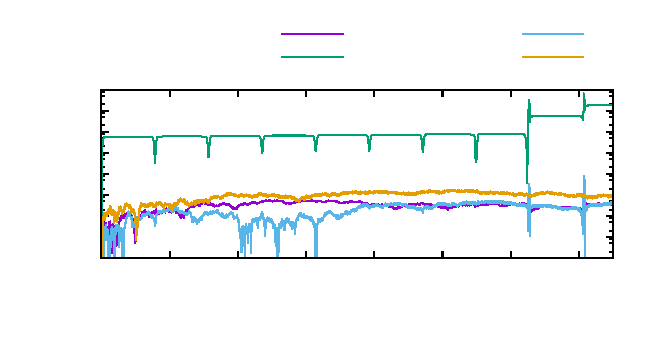
\includegraphics{../latex/plots/deltae}}%
    \gplfronttext
  \end{picture}%
\endgroup
	
\end{figure}
\end{frame}


\begin{frame}
\centering
Number of driver evaluations as function of the timestep
\begin{figure}
	\centering
	\input{plots/drivereval}	
\end{figure}
\end{frame}

\section{Long term accuracy}
\begin{frame}
\frametitle{\thesection. \insertsection}
\begin{itemize}
	\item Simple two-body system
	\item Period \num{0.06} unit time
	\item Motion of sun eliminated by giving it negative initial speed
	\item Runge-Kutta with timestep \num{8e-5}
	\item Gragg-Bulirsch-Stür with timestep \num{1e-3}
\end{itemize}
\end{frame}

\begin{frame}
\centering
10 periods of a simple two-body system
\begin{figure}
	\input{plots/comp_short}	
\end{figure}
\end{frame}


\begin{frame}
\centering
2500 periods of a simple two-body system
\begin{figure}
	% GNUPLOT: LaTeX picture with Postscript
\begingroup
  \makeatletter
  \providecommand\color[2][]{%
    \GenericError{(gnuplot) \space\space\space\@spaces}{%
      Package color not loaded in conjunction with
      terminal option `colourtext'%
    }{See the gnuplot documentation for explanation.%
    }{Either use 'blacktext' in gnuplot or load the package
      color.sty in LaTeX.}%
    \renewcommand\color[2][]{}%
  }%
  \providecommand\includegraphics[2][]{%
    \GenericError{(gnuplot) \space\space\space\@spaces}{%
      Package graphicx or graphics not loaded%
    }{See the gnuplot documentation for explanation.%
    }{The gnuplot epslatex terminal needs graphicx.sty or graphics.sty.}%
    \renewcommand\includegraphics[2][]{}%
  }%
  \providecommand\rotatebox[2]{#2}%
  \@ifundefined{ifGPcolor}{%
    \newif\ifGPcolor
    \GPcolorfalse
  }{}%
  \@ifundefined{ifGPblacktext}{%
    \newif\ifGPblacktext
    \GPblacktexttrue
  }{}%
  % define a \g@addto@macro without @ in the name:
  \let\gplgaddtomacro\g@addto@macro
  % define empty templates for all commands taking text:
  \gdef\gplbacktext{}%
  \gdef\gplfronttext{}%
  \makeatother
  \ifGPblacktext
    % no textcolor at all
    \def\colorrgb#1{}%
    \def\colorgray#1{}%
  \else
    % gray or color?
    \ifGPcolor
      \def\colorrgb#1{\color[rgb]{#1}}%
      \def\colorgray#1{\color[gray]{#1}}%
      \expandafter\def\csname LTw\endcsname{\color{white}}%
      \expandafter\def\csname LTb\endcsname{\color{black}}%
      \expandafter\def\csname LTa\endcsname{\color{black}}%
      \expandafter\def\csname LT0\endcsname{\color[rgb]{1,0,0}}%
      \expandafter\def\csname LT1\endcsname{\color[rgb]{0,1,0}}%
      \expandafter\def\csname LT2\endcsname{\color[rgb]{0,0,1}}%
      \expandafter\def\csname LT3\endcsname{\color[rgb]{1,0,1}}%
      \expandafter\def\csname LT4\endcsname{\color[rgb]{0,1,1}}%
      \expandafter\def\csname LT5\endcsname{\color[rgb]{1,1,0}}%
      \expandafter\def\csname LT6\endcsname{\color[rgb]{0,0,0}}%
      \expandafter\def\csname LT7\endcsname{\color[rgb]{1,0.3,0}}%
      \expandafter\def\csname LT8\endcsname{\color[rgb]{0.5,0.5,0.5}}%
    \else
      % gray
      \def\colorrgb#1{\color{black}}%
      \def\colorgray#1{\color[gray]{#1}}%
      \expandafter\def\csname LTw\endcsname{\color{white}}%
      \expandafter\def\csname LTb\endcsname{\color{black}}%
      \expandafter\def\csname LTa\endcsname{\color{black}}%
      \expandafter\def\csname LT0\endcsname{\color{black}}%
      \expandafter\def\csname LT1\endcsname{\color{black}}%
      \expandafter\def\csname LT2\endcsname{\color{black}}%
      \expandafter\def\csname LT3\endcsname{\color{black}}%
      \expandafter\def\csname LT4\endcsname{\color{black}}%
      \expandafter\def\csname LT5\endcsname{\color{black}}%
      \expandafter\def\csname LT6\endcsname{\color{black}}%
      \expandafter\def\csname LT7\endcsname{\color{black}}%
      \expandafter\def\csname LT8\endcsname{\color{black}}%
    \fi
  \fi
    \setlength{\unitlength}{0.0500bp}%
    \ifx\gptboxheight\undefined%
      \newlength{\gptboxheight}%
      \newlength{\gptboxwidth}%
      \newsavebox{\gptboxtext}%
    \fi%
    \setlength{\fboxrule}{0.5pt}%
    \setlength{\fboxsep}{1pt}%
\begin{picture}(6348.00,3288.00)%
    \gplgaddtomacro\gplbacktext{%
      \csname LTb\endcsname%
      \put(185,1972){\makebox(0,0)[r]{\strut{}$-1$}}%
      \put(185,2260){\makebox(0,0)[r]{\strut{}$-0.5$}}%
      \put(185,2547){\makebox(0,0)[r]{\strut{}$0$}}%
      \put(185,2835){\makebox(0,0)[r]{\strut{}$0.5$}}%
      \put(185,3122){\makebox(0,0)[r]{\strut{}$1$}}%
      \put(317,1752){\makebox(0,0){\strut{}$-1$}}%
      \put(793,1752){\makebox(0,0){\strut{}$-0.5$}}%
      \put(1269,1752){\makebox(0,0){\strut{}$0$}}%
      \put(1745,1752){\makebox(0,0){\strut{}$0.5$}}%
      \put(2221,1752){\makebox(0,0){\strut{}$1$}}%
    }%
    \gplgaddtomacro\gplfronttext{%
      \csname LTb\endcsname%
      \put(1269,3452){\makebox(0,0){\strut{}Positions}}%
    }%
    \gplgaddtomacro\gplbacktext{%
      \csname LTb\endcsname%
      \put(3359,1972){\makebox(0,0)[r]{\strut{}\num{0}}}%
      \put(3359,2228){\makebox(0,0)[r]{\strut{}\num{2e-13}}}%
      \put(3359,2483){\makebox(0,0)[r]{\strut{}\num{4e-13}}}%
      \put(3359,2739){\makebox(0,0)[r]{\strut{}\num{6e-13}}}%
      \put(3359,2994){\makebox(0,0)[r]{\strut{}\num{8e-13}}}%
      \put(3491,1752){\makebox(0,0){\strut{}$0$}}%
      \put(3808,1752){\makebox(0,0){\strut{}$20$}}%
      \put(4126,1752){\makebox(0,0){\strut{}$40$}}%
      \put(4443,1752){\makebox(0,0){\strut{}$60$}}%
      \put(4760,1752){\makebox(0,0){\strut{}$80$}}%
      \put(5077,1752){\makebox(0,0){\strut{}$100$}}%
      \put(5395,1752){\makebox(0,0){\strut{}$120$}}%
      \put(5712,1752){\makebox(0,0){\strut{}$140$}}%
      \put(6029,1752){\makebox(0,0){\strut{}$160$}}%
    }%
    \gplgaddtomacro\gplfronttext{%
      \csname LTb\endcsname%
      \put(4760,3452){\makebox(0,0){\strut{}Energy error}}%
      \csname LTb\endcsname%
      \put(3623,2949){\makebox(0,0)[l]{\strut{}GBS}}%
    }%
    \gplgaddtomacro\gplbacktext{%
      \csname LTb\endcsname%
      \put(185,164){\makebox(0,0)[r]{\strut{}-1}}%
      \put(185,452){\makebox(0,0)[r]{\strut{}-0.5}}%
      \put(185,739){\makebox(0,0)[r]{\strut{}0}}%
      \put(185,1027){\makebox(0,0)[r]{\strut{}0.5}}%
      \put(185,1314){\makebox(0,0)[r]{\strut{}1}}%
      \put(317,-56){\makebox(0,0){\strut{}$-1$}}%
      \put(793,-56){\makebox(0,0){\strut{}$-0.5$}}%
      \put(1269,-56){\makebox(0,0){\strut{}$0$}}%
      \put(1745,-56){\makebox(0,0){\strut{}$0.5$}}%
      \put(2221,-56){\makebox(0,0){\strut{}$1$}}%
    }%
    \gplgaddtomacro\gplfronttext{%
    }%
    \gplgaddtomacro\gplbacktext{%
      \csname LTb\endcsname%
      \put(3359,164){\makebox(0,0)[r]{\strut{}\num{0}}}%
      \put(3359,493){\makebox(0,0)[r]{\strut{}\num{4e-09}}}%
      \put(3359,821){\makebox(0,0)[r]{\strut{}\num{8e-09}}}%
      \put(3359,1150){\makebox(0,0)[r]{\strut{}\num{1.2e-08}}}%
      \put(3491,-56){\makebox(0,0){\strut{}$0$}}%
      \put(3808,-56){\makebox(0,0){\strut{}$20$}}%
      \put(4126,-56){\makebox(0,0){\strut{}$40$}}%
      \put(4443,-56){\makebox(0,0){\strut{}$60$}}%
      \put(4760,-56){\makebox(0,0){\strut{}$80$}}%
      \put(5077,-56){\makebox(0,0){\strut{}$100$}}%
      \put(5395,-56){\makebox(0,0){\strut{}$120$}}%
      \put(5712,-56){\makebox(0,0){\strut{}$140$}}%
      \put(6029,-56){\makebox(0,0){\strut{}$160$}}%
    }%
    \gplgaddtomacro\gplfronttext{%
      \csname LTb\endcsname%
      \put(3623,1141){\makebox(0,0)[l]{\strut{}RK}}%
    }%
    \gplbacktext
    \put(0,0){\includegraphics{../latex/plots/comp_long}}%
    \gplfronttext
  \end{picture}%
\endgroup
	
\end{figure}	
\end{frame}


\section{Adaptive timestep}
\begin{frame}
\frametitle{\thesection. \insertsection}
\centering
\vspace{-0.3cm}
Burrau problem with \emph{no} adaptive timestep
\includemedia[
  activate=onclick,
  width=10cm,
  height=6.5cm,
  keepaspectratio,
  addresource=movies/burraunon.mp4,
  flashvars={source=movies/burraunon.mp4&autoPlay=false&scaleMode=none&loop=false}  
]{\includegraphics{rkwit}}{VPlayer.swf}
\end{frame}

\begin{frame}
\centering
Burrau problem \emph{with} adaptive timestep
\includemedia[
  activate=onclick,
  width=10cm,
  height=6.5cm,
  keepaspectratio,
  addresource=movies/burrauadap.mp4,
  flashvars={source=movies/burrauadap.mp4&autoPlay=false&scaleMode=none&loop=false}  
]{\includegraphics{rkadapwit}}{VPlayer.swf}	
\end{frame}


\section{Choreographies}
\begin{frame}
\frametitle{\thesection. \insertsection}
\vspace{-0.3cm}
\centering
Three-body choreographies with RK timestep \num{e-4}
\begin{figure}
	\input{plots/choreographies}	
\end{figure}
\end{frame}

%\begin{frame}
%\vspace{-0.5cm}
%\centering
%\includemedia[
%  activate=onclick,
%  width=9cm,
%  height=6cm,
%  keepaspectratio,
%  addresource=movies/burrau.mp4,
%  flashvars={source=movies/burrau.mp4&autoPlay=false&scaleMode=none&loop=false}  
%]{\includegraphics{desk}}{VPlayer.swf}	
%\end{frame}


\begin{frame}
\centering
\vspace{-0.5cm}
\includemedia[
  activate=onclick,
  width=12.5cm,
  height=7cm,
  keepaspectratio,
  addresource=movies/yin4.mp4,
  flashvars={source=movies/yin4.mp4&autoPlay=false&scaleMode=none&loop=false}  
]{\includegraphics{yinyang}}{VPlayer.swf}
\end{frame}
	
	
\begin{frame}
\centering
\includemedia[
  activate=onclick,
  width=11cm,
  height=7.5cm,
  keepaspectratio,
  addresource=movies/butterfly.mp4,
  flashvars={source=movies/butterfly.mp4&autoPlay=false&scaleMode=none&loop=false}  
]{\includegraphics{butterfly}}{VPlayer.swf}	
\end{frame}

\end{document}